\documentclass[a4paper,11pt]{article}
\usepackage{amsmath}

\usepackage[utf8]{inputenc}
\usepackage{pgfplots}
\pgfplotsset{compat=1.17}
\usepackage{graphicx}
\usepackage{float}
\usepackage{graphicx}
\usepackage{caption}
\usepackage{subcaption}

\usepackage{hyperref}

\usepackage{pgfplots}
\pgfplotsset{compat=1.18} 

\usepackage{minted}

\begin{document}

\title{
    \textbf{Assignment 2 Report - Programming with OpenMP}
}
\author{Dean Tsankov, Kacper Lisik}
\date{\today}

\maketitle

\section*{Introduction}

In this assignment, we learn how to write, build and execute a parallel program in OpenMP to show performance speedup on more than one processor as well as to find dependencies in loops and to write code such that it can correctly be executed in parallel.

\section*{Problem 1 - Compute the Sum, Min, and Max of Matrix Elements}

To begin with we are given the matrixSum-openmp.c program which we have to manipulate in order to complete the given tasks as an introduction to OpenMP directives.

\subsection*{Task description}

\begin{minted}[
frame=single,
framesep=2mm,
baselinestretch=1.2,
fontsize=\footnotesize,
breaklines,
]{text}
The purpose of this problem is to introduce us to basic OpenMP usage. The program matrixSum-openmp.c computes a sum of matrix elements in parallel using OpenMP. Develop and evaluate the following modified version of the program.
Extend the program so that in addition to the sum, it finds and prints a value and a position (indexes) of the maximum element of the matrix and a value and a position of the minimum element of the matrix. To check your solution, initialize elements of the matrix to random values. Use OpenMP constructs. Run the program on different numbers of processors and report the speedup (sequential execution time divided by parallel execution time) for different numbers of processors (up to at least 4) and different sizes of matrices (at least 3 different sizes). Run each program several (at least 5) times and use the median value for execution time. Try to provide reasonable explanations for your results. Measure only the parallel part of your program.
\end{minted}


\subsection*{Key points of solution}
OpenMp makes it very simple to turn a sequential implementation of a program into a concurrent one. The traversal loop over the matrix looks like so:

\begin{minted}[
frame=single,
framesep=2mm,
baselinestretch=1.2,
fontsize=\footnotesize,
]{c}
    (...)
    start_time = omp_get_wtime();
    #pragma omp parallel for reduction(+ : total) private(j) shared(min,max)
        for (i = 0; i < size; i++){
            for (j = 0; j < size; j++)
            {
                total += matrix[i][j];
                if (matrix[i][j] < min.value)
                {
                    min.value = matrix[i][j];
                    min.xCoordinate = j;
                    min.yCoordinate = i;
                }
                else if (matrix[i][j] > max.value)
                {
                    max.value = matrix[i][j];
                    max.xCoordinate = j;
                    max.yCoordinate = i;
                }
            }
        }
        // implicit barrier

        end_time = omp_get_wtime();
    (...)
\end{minted}

\subsection*{Performance exploration}

Example sequential time as a median from 100 executions for an 8x8 matrix: \[ 8.73899 * 10^{-8}s\]

\begin{figure}[H]
    \centering
    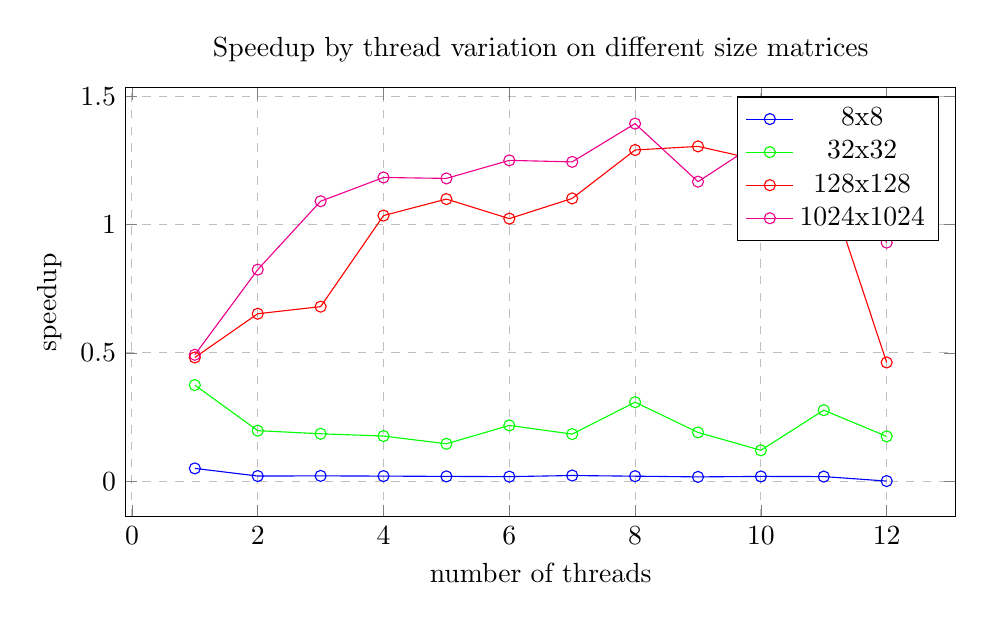
\begin{tikzpicture}
        \begin{axis}[
            title={Speedup by thread variation on different size matrices},
            width=\linewidth,
            height=200,
            xlabel={number of threads},
            ylabel={speedup},
            ymajorgrids=true,
            xmajorgrids=true,
            grid style=dashed,
        ]
        
        \addplot[
            color=blue,
            mark=o,
            ]
            coordinates {
           (1, 0.0503607)(2, 0.0205732)(3, 0.0212526)(4, 0.0203416)(5, 0.0192045)(6, 0.0182709)(7, 0.0226081)(8, 0.0200073)(9, 0.0173001)(10, 0.0191062)(11, 0.0184819)(12, 0.000992439)

            };
            \addlegendentry{8x8}

        \addplot[
            color=green,
            mark=o,
            ]
            coordinates {
            (1, 0.374876)(2, 0.197327)(3, 0.185149)(4, 0.176334)(5, 0.146219)(6, 0.217691)(7, 0.183862)(8, 0.308297)(9, 0.190484)(10, 0.120867)(11, 0.277114)(12, 0.174977)
            };
            \addlegendentry{32x32}

        \addplot[
            color=red,
            mark=o,
            ]
            coordinates {
            (1, 0.482204)(2, 0.652608)(3, 0.680176)(4, 1.03481)(5, 1.09904)(6, 1.0229)(7, 1.10154)(8, 1.29014)(9, 1.30424)(10, 1.24907)(11, 1.20019)(12, 0.462933)
            };
            \addlegendentry{128x128}

        \addplot[
            color=magenta,
            mark=o,
            ]
            coordinates {
            (1, 0.492763)(2, 0.824244)(3, 1.09068)(4, 1.18312)(5, 1.1795)(6, 1.24978)(7, 1.24385)(8, 1.39286)(9, 1.16681)(10, 1.3264)(11, 1.35838)(12, 0.929522)
            };
            \addlegendentry{1024x1024}
        \end{axis}
        \end{tikzpicture}
    \caption{Tree add time complexity}
    \label{fig:plot1}
\end{figure}

Generally we would expect the speedup to keep increasing not decrease. Still these results could make sense considering that parallelizing helps for big workloads, or when the workers are used many times over for many moderate sized tasks (so the cost of launching the threads is a fraction of the work they do). But in this case performing an objectively small amount of additions and comparisons it is negligible to the CPU. And so they are just not doing enough to benefit from parallelizing this specific task.


\section*{Problem 2 - Quicksort}

\subsection*{Task description}

\begin{minted}[
frame=single,
framesep=2mm,
baselinestretch=1.2,
fontsize=\footnotesize,
breaklines,
]{text}
The quicksort algorithm sorts the list of numbers by first dividing the list into two sublists so that all the numbers if one sublist are smaller than all the numbers in the other sublist. This is done by selecting one number (called a pivot) against which all other numbers are compared: the numbers which are less than the pivot are placed in one sublist, and the numbers which more than the pivot are placed in another sublist. The pivot can be either placed in one sublist or withheld and placed in its final position. Develop a parallel multithreaded program (in C/C++ using OpenMP tasks) with recursive parallelism that implements the quicksort algorithm for sorting an array of n values. Perform speedup tests on the parallel part of the code and give explinations.
\end{minted}

\subsection*{Key points of solution}

Following the standard procedure of developing a quicksort algorithm we just have to introduce the proper opemmp directives in crucial spots in order to make the recursive calls of the algorithm execute on separate threads and as such parallelize the execution. The entire code can be found in the source code directory, here is the main openmp section

\begin{minted}[
frame=single,
framesep=2mm,
baselinestretch=1.2,
fontsize=\footnotesize,
]{c}
    (...)
    Array quickSort(Array *mainSet)
    {
        Array left;
        Array right;
        for (k = 0; k < currSize; k++)
        {
            if (mainSet->array[k] < pivot)
            {
                insertArray(&left, mainSet->array[k]);
            }
            else if (mainSet->array[k] > pivot)
            {
                insertArray(&right, mainSet->array[k]);
            }
            (...)
        }
        
        #pragma omp task shared(left)
        {
            left = quickSort(&left);
        }
        
        #pragma omp task shared(right)
        {
            right = quickSort(&right);
        }
        
        #pragma omp taskwait
        (...)
    }
    (...)
\end{minted}

We have to use {\tt omp taskwait} in order to ensure that all previously generated calls were executed before we can continue on joining the left and right parts of the set.

Another important note is that at the first {\tt quicksort()} function call we need to initialize a parallel space as:

\begin{minted}[
frame=single,
framesep=2mm,
baselinestretch=1.2,
fontsize=\footnotesize,
]{c}
    (...)
    start_time = omp_get_wtime();
    #pragma omp parallel
    {
        #pragma omp single
        {
            sorted = quickSort(&toSortSet);
        }
    }
    end_time = omp_get_wtime();
    (...)
\end{minted}

We then run the initial call as single so as to let the other threads be ready to begin working on the tasks spawned by the original single thread.

\subsection*{Performance exploration}


\begin{figure}[H]
    \centering
    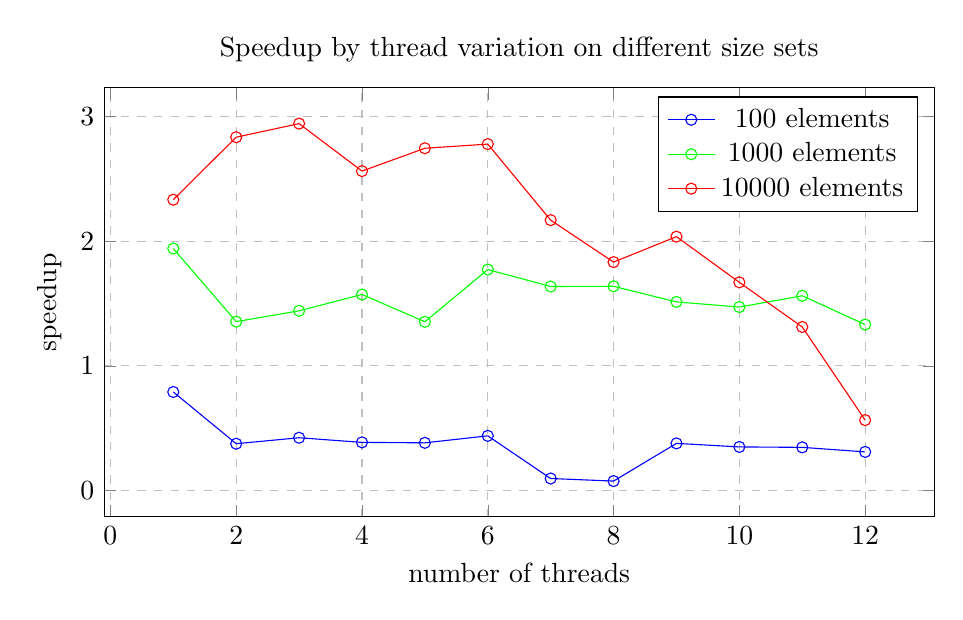
\begin{tikzpicture}
        \begin{axis}[
            title={Speedup by thread variation on different size sets},
            width=\linewidth,
            height=200,
            xlabel={number of threads},
            ylabel={speedup},
            ymajorgrids=true,
            xmajorgrids=true,
            grid style=dashed,
        ]
        
        \addplot[
            color=blue,
            mark=o,
            ]
            coordinates {
            (1, 0.790388)(2, 0.375346)(3, 0.423195)(4, 0.385974)(5, 0.382457)(6, 0.4384)(7, 0.0961835)(8, 0.0755478)(9, 0.377974)(10, 0.349614)(11, 0.346003)(12, 0.309711)
            };
            \addlegendentry{100 elements}

        \addplot[
            color=green,
            mark=o,
            ]
            coordinates {
            (1, 1.94086)(2, 1.35466)(3, 1.44125)(4, 1.57234)(5, 1.35354)(6, 1.77238)(7, 1.63637)(8, 1.63805)(9, 1.51279)(10, 1.47141)(11, 1.56183)(12, 1.3308)
            };
            \addlegendentry{1000 elements}

        \addplot[
            color=red,
            mark=o,
            ]
            coordinates {
            (1, 2.3326)(2, 2.83397)(3, 2.94283)(4, 2.56206)(5, 2.74519)(6, 2.7785)(7, 2.16856)(8, 1.83208)(9, 2.03614)(10, 1.66971)(11, 1.31167)(12, 0.564774)
            };
            \addlegendentry{10000 elements}
        \end{axis}
        \end{tikzpicture}
    \caption{Tree add time complexity}
    \label{fig:plot1}
\end{figure}
Here it is unclear to us why the openmp single thread execution still has a noticeable speedup, but we could probably assume that this is just a standard offset due to the variation in the generated data. Otherwise the trends seem to follow the notion that there is a threshold at which creating more threads is more computationally intensive then the positive work done by them in total. Not to mention the fact that the computer on which these tests were ran has 6 physical cores and 12 logical processors so the downward trend after 6 threads could also have to do with the hardware implementation.



\section*{Problem 6 - Find Palindromes and Semordnilaps}
\begin{minted}[
frame=single,
framesep=2mm,
baselinestretch=1.2,
fontsize=\footnotesize,
breaklines,
]{text}
There is an online dictionary in /usr/dict/words or /usr/share/dict/words under Linux. The file is used, in particular, by the Linux spell command and contains a few thousand words, e.g., 235886 words. You can download a smaller file called words containing 25143 words.
Recall that palindromes are words or phrases that read the same forward and backward, such as "noon" or "radar," i.e., if you reverse all the letters, you get the same word or phrase. Reverse pairs or semordnilaps are words whose reverse forms are different valid words, such as "draw" and "ward". Your task is to find all palindromes and all  semordnilaps in the dictionary. For example, "noon" is a palindrome; hence, its reverse is trivially in the dictionary. A word like "draw" is semordnilap and "ward" is also in the dictionary.
Your parallel program should use W worker processes, where W is a command-line argument. Use the workers just for the compute phase (i.e., to find the palindromic words); do the input and output phases sequentially. Each worker should count the number of words (palindromes and semordnilaps) that it finds. Your program should write the palindromes and semordnilaps to a results file and output the total number of palindromes and semordnilaps in the dictionary and the number of palindromes and semordnilaps found by each worker.
\end{minted}


\subsection*{Key points of solution}
After sequentially reading the words file, we ensure that the words are sorted in alphabetical order. They appear to be sorted, but to be certain, we use the \texttt{std::sort()} command, which is computationally inexpensive if the words are already sorted or nearly sorted. We distribute the work and create $N$ threads, with each thread checking whether any of $\text{num\_of\_words} / \text{num\_of\_threads}$ words is a palindrome or a semordnilap:
\newpage
\begin{minted}[
frame=single,
framesep=2mm,
baselinestretch=1.2,
fontsize=\footnotesize,
]{c}
(...)
    #pragma omp parallel
    {
        int thread_id = omp_get_thread_num();
        thrd_data[thread_id].start = (words.size()/workers) * thread_id;
        thrd_data[thread_id].end = (thread_id == workers - 1)? 
            words.size()-1 : (words.size()/workers) * (thread_id+1);
        thrd_data[thread_id].tid = thread_id;
        thread_fun(&thrd_data[thread_id]);
    }
(...)
\end{minted}

Thread function:

\begin{minted}[
frame=single,
framesep=2mm,
baselinestretch=1.2,
fontsize=\footnotesize,
]{c}
(...)
void* thread_fun (thread_data* data){
    data->palindromes = 0;
    data->semordnilaps = 0;
    for (int i = data->start; i < data->end; i++){
        //calculate the reverse
        string reverse = words[i];
        for (int j = 0; j < reverse.size() / 2; j++)
            swap(reverse[j], reverse[reverse.size() - 1 - j]); 

        //check if palindrome
        if(compare_strings(reverse, words[i]) == 0){
            data->palindromes_vector.pb(reverse);
            data->palindromes++;
            continue;
        }

        //look for semordnilaps - fast
        int result;
        if((result = binsearch(i+1,words.size()-1, reverse)) != -1){
            data->semordnilaps_vector.pb(words[result]);
            data->semordnilaps_vector.pb(words[i]);
            data->semordnilaps+=2;
        } 
    }
    return NULL;
}
(...)
\end{minted}

Each thread goes through its assigned list of words, computes the reverse of every word, and checks if the word is a palindrome. Then, using binary search, it looks through the word list to see if the reverse of the given word is also in the word list.



\subsection*{Parallel Performance Analysis}
\subsubsection*{Experiment Setup}

To analyze the speedup of the palindrome detection program, we ran the experiment on three different dictionary sizes:
\begin{itemize}
    \item \textbf{Small Dictionary} (2,514 words)
    \item \textbf{Medium Dictionary} (8,381 words)
    \item \textbf{Large Dictionary} (25,143 words)
\end{itemize}

For each dictionary size, we ran the program with \textbf{1, 2, 4, and 8 threads}.  
Each configuration was executed \textbf{50 times}, and the median execution time was used to calculate the speedup:

\[
\text{Speedup} = \frac{\text{Sequential Time}}{\text{Parallel Time}}
\]

\subsubsection*{Results and Discussion}

\begin{figure}[H]
    \centering
    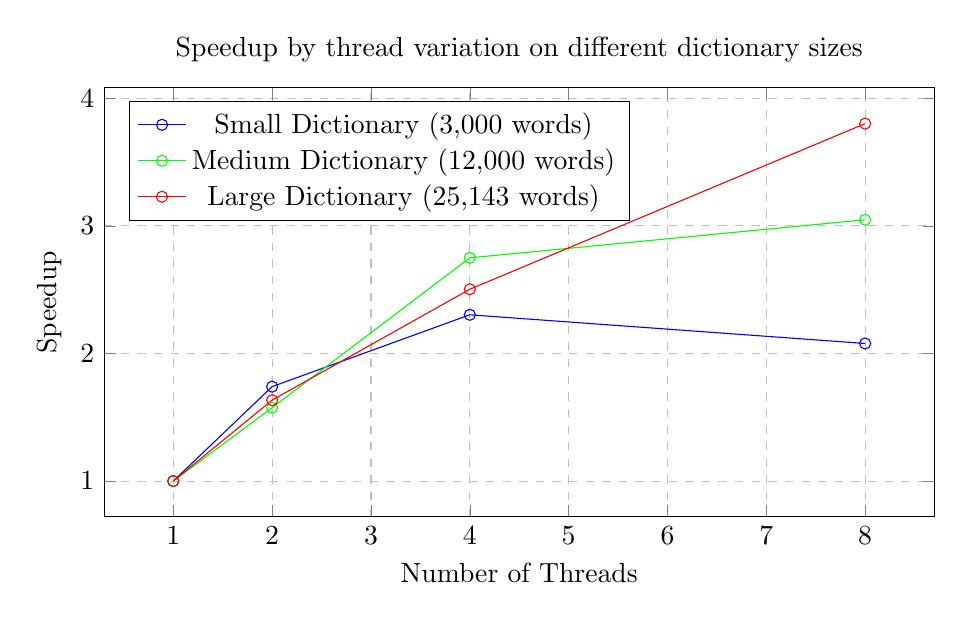
\begin{tikzpicture}
        \begin{axis}[
            title={Speedup by thread variation on different dictionary sizes},
            width=\linewidth,
            height=200,
            xlabel={Number of Threads},
            ylabel={Speedup},
            ymajorgrids=true,
            xmajorgrids=true,
            grid style=dashed,
            legend pos=north west
        ]
        
        \addplot[
            color=blue,
            mark=o,
            ]
            coordinates {
            (1, 1.0) (2, 1.739939) (4, 2.302861) (8, 2.078192)
            };
            \addlegendentry{Small Dictionary (3,000 words)}

        \addplot[
            color=green,
            mark=o,
            ]
            coordinates {
            (1, 1.0) (2, 1.575115) (4, 2.749119) (8, 3.047419)
            };
            \addlegendentry{Medium Dictionary (12,000 words)}

        \addplot[
            color=red,
            mark=o,
            ]
            coordinates {
            (1, 1.0) (2, 1.633946) (4, 2.502834) (8, 3.800739)
            };
            \addlegendentry{Large Dictionary (25,143 words)}
        \end{axis}
    \end{tikzpicture}
    \caption{Speedup for different dictionary sizes}
    \label{fig:speedup}
\end{figure}

\subsubsection*{Analysis of Results}

The speedup increases as we add more threads, but the improvement is not perfectly linear due to \textbf{parallel overhead} and \textbf{synchronization costs}.  

\begin{itemize}
    \item \textbf{For 2 threads}: Speedup is between 1.5x–1.7x, showing a good improvement.  
    \item \textbf{For 4 threads}: Speedup increases to 2.3x–2.7x, demonstrating good parallel efficiency.  
    \item \textbf{For 8 threads}: Speedup \textbf{flattens for the small and medium dictionaries}, meaning adding more threads does not improve performance much. This is likely because:
    \begin{itemize}
        \item The extra threads \textbf{spend more time managing work} than actually processing words.
        \item \textbf{Memory access slows down} when too many threads try to read and write at the same time.
        \item The workload is \textbf{too small to be efficiently split} among all threads.
    \end{itemize}

\end{itemize}

\subsubsection*{Conclusion}

\begin{itemize}
    \item \textbf{Smaller dictionaries} show \textbf{less speedup} because parallel overhead is relatively large compared to the computational cost.  
    \item \textbf{Larger dictionaries} benefit more from parallelism, but the gains diminish as the number of threads increases.  
\end{itemize}
\end{document}